%**************** TESTS FOR THE CODE ******************
\section{Tests on Synthetic Graphs}
\label{sec5.2}
\subsection{Stochastic Block Model Test Graph}
To start testing our code we choose a Stochastic Block Model (SBM) graph. A SBM graph is a type of random graph model used to generate networks with a predefined community structure. It is an extension of the Erdos--R\'enyi, where nodes are divided into communities, and the probability of an edge between two nodes depends on their community membership. It is characterized by \textit{N} nodes, \textit{k} communities and a connectivity matrix \textit{$P_{ij}$} which represents the probability of an edge between a node in community $i$ and a node in community $j$.
Since communities are predefined when generating the graph, we can directly compare the detected communities with the true ones.

For our test we set 
\begin{equation*}
    N = 500, \quad k = 2, \quad
    P =
    \begin{bmatrix} 
        0.20 & 0.03 \\
        0.03 & 0.20
    \end{bmatrix}
\end{equation*}
with every initial weight equal to one.

\begin{figure}
    \centering
    \begin{subfigure}{0.45\textwidth}
        \centering
        \includegraphics[width=\textwidth]{../tests/ToyModelResults/SBM/Before Ricci Flow.png}
        \caption{Initial SBM graph, before Ricci Flow.}
    \end{subfigure}
    \hfill
    \begin{subfigure}{0.45\textwidth}
        \centering
        \includegraphics[width=\textwidth]{../tests/ToyModelResults/SBM/After Ricci Flow.png}
        \caption{SBM graph after Ricci Flow.}
    \end{subfigure}
    \caption{Comparison of SBM graph before and after having applied Ricci Flow on edges.}
\end{figure}
\label{fig:SBM_comparison}

\begin{figure}
    \centering
    \includegraphics[width=0.6\textwidth]{../tests/ToyModelResults/SBM/Surgery Accuracy.png}
    \caption{SBM acc}
\end{figure}
\label{fig:SBM_Accuracy}

\begin{figure}
    \centering
    \begin{subfigure}{0.45\textwidth}
        \centering
        \includegraphics[width=\textwidth]{../tests/ToyModelResults/SBM/After Surgery.png}
        \caption{Final SBM graph, after surgery process.}
    \end{subfigure}
    \hfill
    \begin{subfigure}{0.45\textwidth}
        \centering
        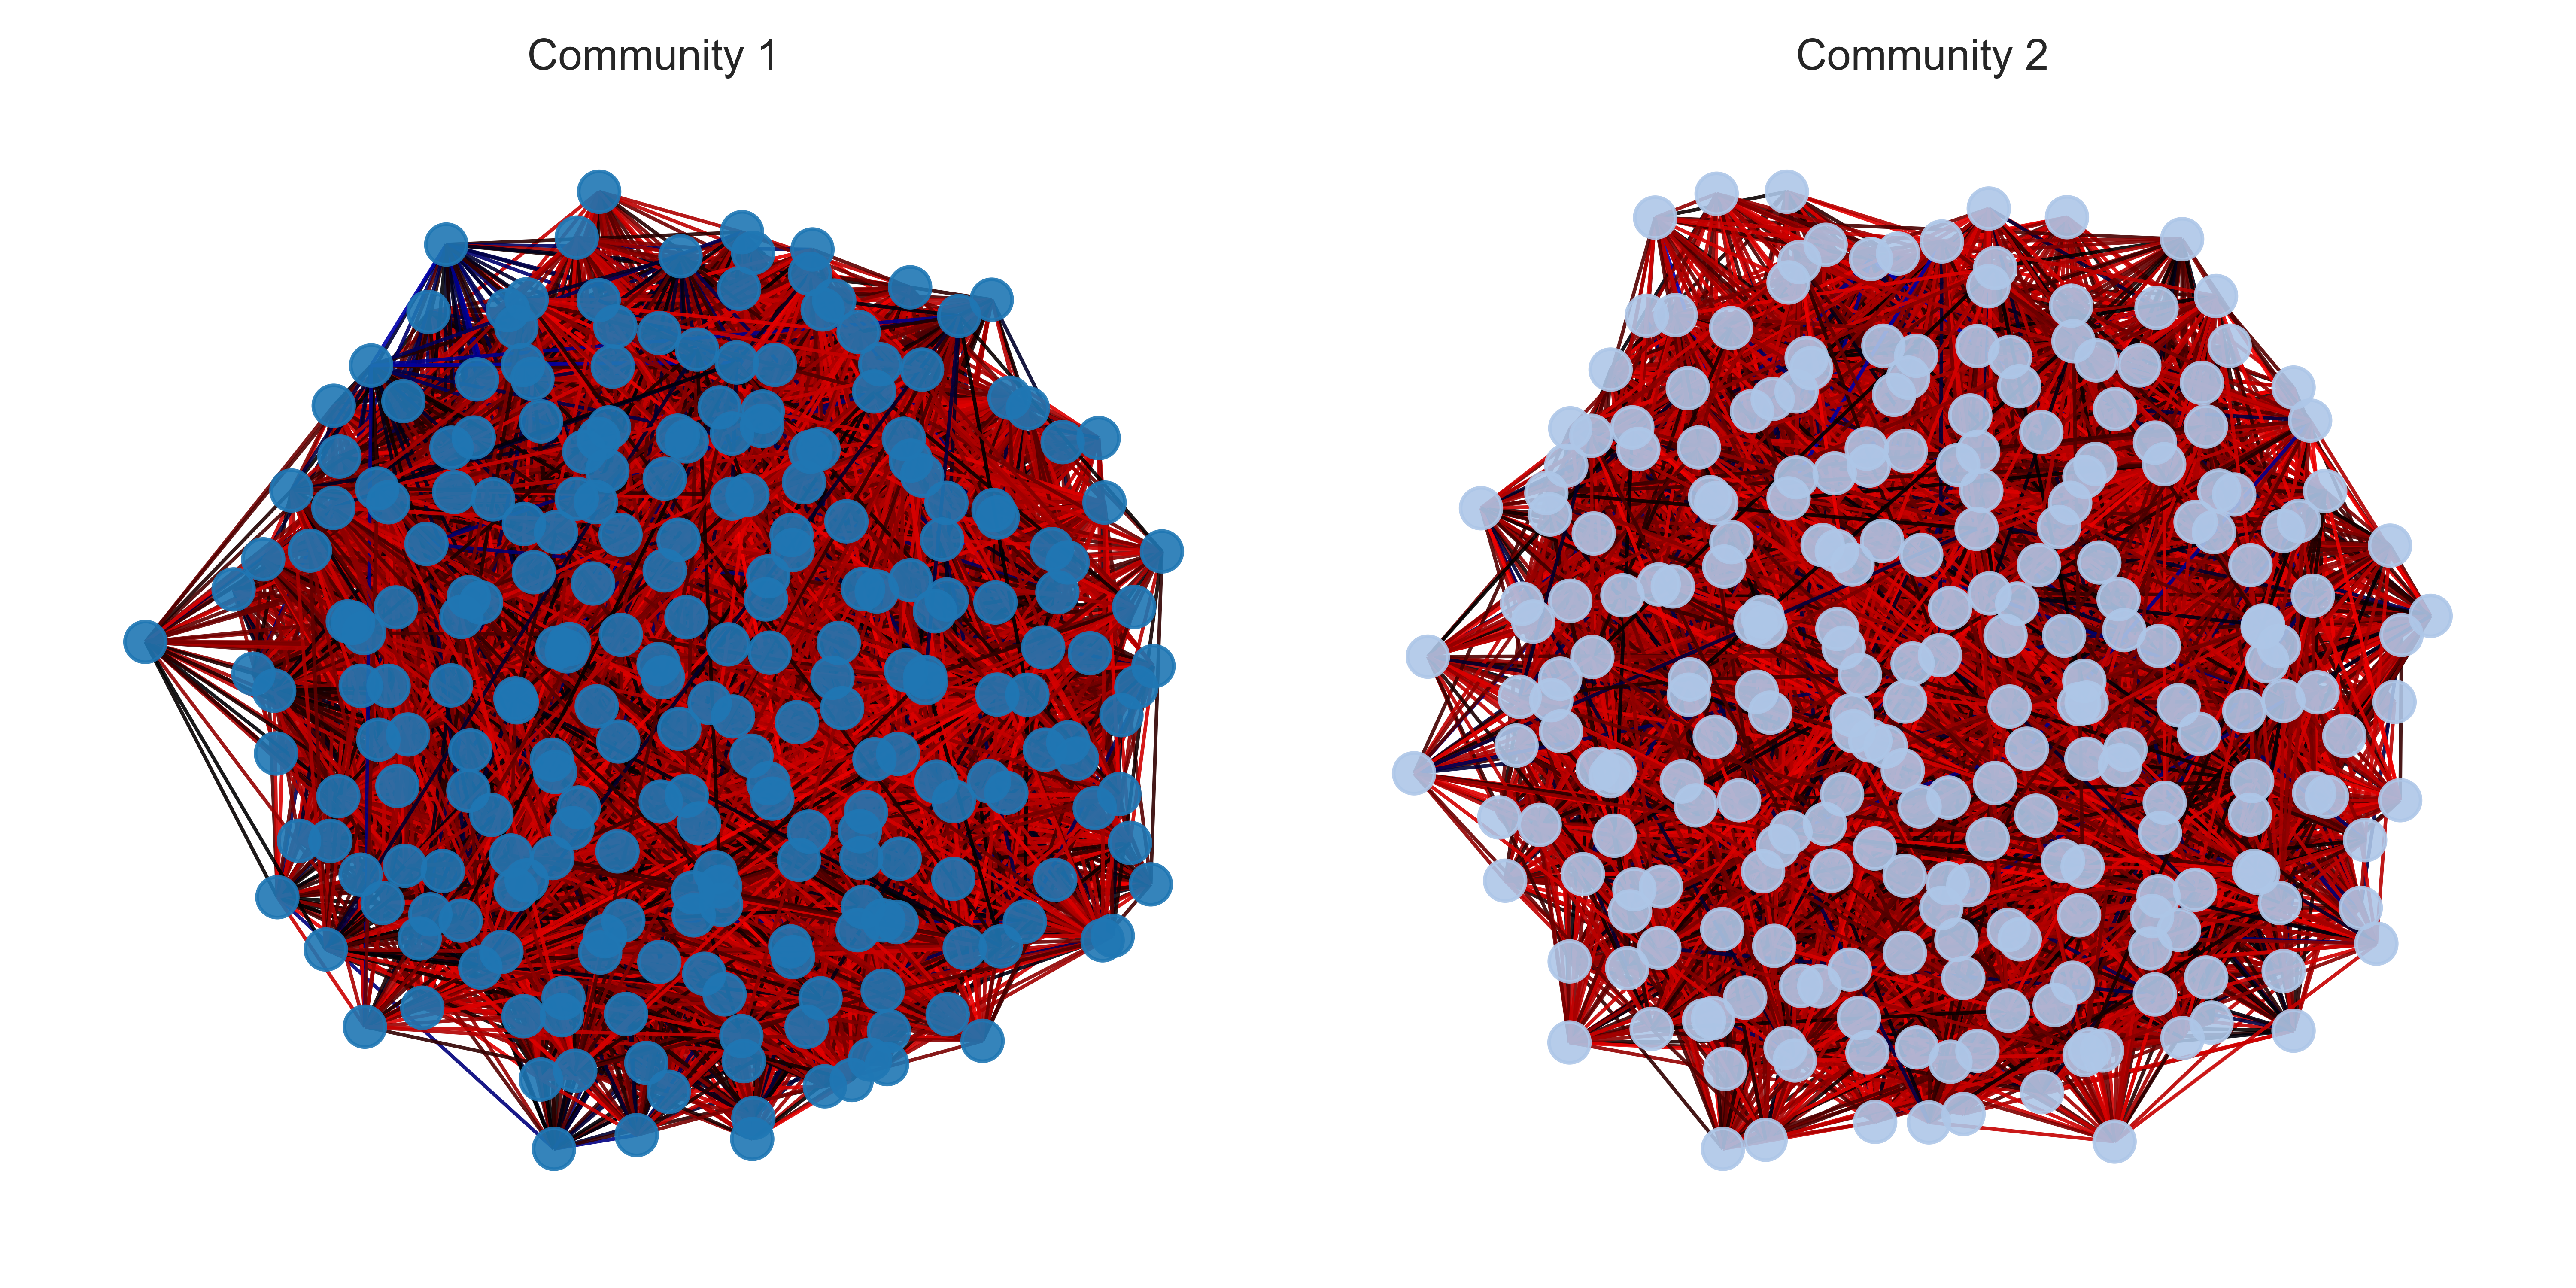
\includegraphics[width=\textwidth]{../tests/ToyModelResults/SBM/Detected Communities.png}
        \caption{Detected communities after surgery on SBM graph.}
    \end{subfigure}
    \caption{Comparison of SBM graph after surgery and corrensponding connected components (i.e. the detected communities).}
\end{figure}
\label{fig:SBM_Communities}


\subsection{Lancichinetti-Fortunato-Radicchi Test Graph}
Lancichinetti-Fortunato-Radicchi (LFR)

\begin{figure}
    \centering
    \begin{subfigure}{0.45\textwidth}
        \centering
        \includegraphics[width=\textwidth]{../tests/ToyModelResults/LFR/Before Ricci Flow.png}
        \caption{Initial LFR graph, before Ricci Flow.}
    \end{subfigure}
    \hfill
    \begin{subfigure}{0.45\textwidth}
        \centering
        \includegraphics[width=\textwidth]{../tests/ToyModelResults/LFR/After Ricci Flow.png}
        \caption{LFR graph after Ricci Flow.}
    \end{subfigure}
    \caption{Comparison of LFR graph before and after having applied Ricci Flow on edges.}
\end{figure}
\label{fig:LFR_comparison}


\begin{figure}
    \centering
    \includegraphics[width=0.6\textwidth]{../tests/ToyModelResults/LFR/Surgery Accuracy.png}
    \caption{LFR acc}
\end{figure}
\label{fig:LFR_Accuracy}

\begin{figure}
    \centering
    \includegraphics[width=0.6\textwidth]{../tests/ToyModelResults/LFR/After Surgery.png}
        \caption{Final LFR graph, after surgery process.}
\end{figure}
\label{fig:LFR_Surgery}

\subsection{Further Tests on Lancichinetti-Fortunato-Radicchi Graphs}

\begin{figure}
    \centering
    \includegraphics[width=0.6\textwidth]{../tests/LFRResults/LFR_OTD.png}
    \caption{LFR OTD}
\end{figure}
\label{fig:LFR_OTD}

\begin{figure}
    \centering
    \includegraphics[width=0.6\textwidth]{../tests/LFRResults/LFR_ATD.png}
    \caption{LFR ATD}
\end{figure}
\label{fig:LFR_ATD}